\documentclass[11pt,a4paper]{article}
\usepackage[margin=2.5cm]{geometry}
\usepackage{amsmath,amssymb}
\usepackage{graphicx,booktabs,listings,xcolor,fancyhdr,hyperref,float,array,setspace}
\hypersetup{colorlinks=true,linkcolor=black,urlcolor=blue}
\setstretch{1.15}
\lstset{language=Verilog,basicstyle=\ttfamily\scriptsize,keywordstyle=\color{blue!60!black},
 commentstyle=\color{green!40!black},numbers=left,numberstyle=\tiny,frame=single,breaklines=true,
 tabsize=2,showstringspaces=false}
\pagestyle{fancy}\fancyhf{}
\fancyhead[L]{32-bit ALU using Verilog}\fancyhead[R]{NIT Srinagar}\fancyfoot[C]{\thepage}

\begin{document}
\begin{titlepage}
\centering
{\large\bfseries NATIONAL INSTITUTE OF TECHNOLOGY SRINAGAR\par}
\vspace{0.3cm}{\large Department of Electronics and Communication Engineering\par}
\vspace{2.5cm}
{\LARGE\bfseries Design and Implementation of a\\32-bit Arithmetic Logic Unit\\using Verilog HDL\par}
\vspace{0.8cm}{\large Mini Project Report\par}
\vspace{3cm}
{\large\bfseries Submitted by\par}\vspace{0.4cm}
{\large Mohammad Irtiqa Bhat\par (2024-25MECECS005)\par}\vspace{0.3cm}
{\large Mohammad Abbas\par (2025MECECS002)\par}
\vfill
{\large Department of Electronics and Communication Engineering\par
National Institute of Technology Srinagar\par}
\vspace{0.5cm}{\large 2026\par}
\end{titlepage}

\begin{abstract}
This report presents the design, implementation and verification of a 32-bit Arithmetic Logic Unit (ALU) in Verilog HDL. The ALU performs sixteen arithmetic, logic, shift and compare operations and produces four status flags: Zero, Negative, Carry and Overflow. The adder is built structurally from eight 4-bit carry-lookahead blocks, shifting is done by a five-stage barrel shifter, and the compare operations re-use the subtractor so that no separate comparator is needed. The design is verified with self-checking testbenches that combine an independent behavioural reference model, directed corner-case tests, constrained-random tests and golden vectors generated by a Python model. Yosys scripts are provided for generic gate-level and Lattice ECP5 synthesis.
\end{abstract}

\tableofcontents
\newpage

%------------------------------------------------------------
\section{Introduction}
The Arithmetic Logic Unit is the computational core of every processor. It receives two operands and an operation code, and produces a result together with flags that describe the outcome. Every instruction that adds, compares, masks bits or shifts a value is executed by the ALU, so its design decides both the functional behaviour and, to a large extent, the clock speed of a processor.

\subsection{Objectives}
\begin{itemize}
\item Design a 32-bit ALU supporting arithmetic, logic, shift and compare operations.
\item Generate the Zero, Negative, Carry and Overflow flags correctly for signed and unsigned data.
\item Implement the design in synthesisable Verilog-2005 using a modular, hierarchical structure.
\item Verify the design with self-checking testbenches and an independent reference model.
\end{itemize}

\subsection{Tools}
Verilog-2005 as the hardware description language; Icarus Verilog and GTKWave for simulation and waveform viewing; Python~3 for the reference model and vector generation; Yosys for synthesis.

%------------------------------------------------------------
\section{Theory}
\subsection{Two's complement arithmetic}
Signed integers are stored in two's complement, so the same adder handles signed and unsigned operands. In 32 bits the signed range is $-2^{31}$ to $2^{31}-1$. Subtraction is performed as
\[ A - B = A + \overline{B} + 1 . \]

\subsection{Carry-lookahead addition}
In a ripple-carry adder each stage waits for the carry of the previous stage, so the delay grows linearly with the word length. A carry-lookahead adder removes this wait by forming the carries directly from two signals per bit, the \emph{propagate} $p_i = a_i \oplus b_i$ and the \emph{generate} $g_i = a_i b_i$. For a 4-bit block with carry-in $c_0$:
\begin{align*}
c_1 &= g_0 + p_0 c_0\\
c_2 &= g_1 + p_1 g_0 + p_1 p_0 c_0\\
c_3 &= g_2 + p_2 g_1 + p_2 p_1 g_0 + p_2 p_1 p_0 c_0\\
c_4 &= g_3 + p_3 g_2 + p_3 p_2 g_1 + p_3 p_2 p_1 g_0 + p_3 p_2 p_1 p_0 c_0\\
s_i &= p_i \oplus c_i
\end{align*}
The 32-bit adder in this project chains eight such 4-bit blocks. Inside a block the carries are fully looked ahead, while between blocks the carry ripples, which is a common compromise between area and speed.

\subsection{Status flags}
\begin{table}[H]\centering
\begin{tabular}{@{}lll@{}}\toprule
Flag & Meaning & Condition\\\midrule
Z & Zero & result $=0$\\
N & Negative & result[31] $=1$\\
C & Carry & carry out of the adder (for subtraction, $C=1$ means no borrow)\\
V & Overflow & operands have equal sign, result has the opposite sign\\\bottomrule
\end{tabular}
\caption{Status flags. C and V are defined for ADD, SUB, INC and DEC only.}
\end{table}

\subsection{Comparison using the subtractor}
The compare operations compute $A + \overline{B} + 1$ and inspect the flags. For signed numbers, $A<B$ exactly when $N \oplus V = 1$. For unsigned numbers, $A<B$ exactly when a borrow occurs, that is when $C=0$. This saves a dedicated comparator.

\subsection{Barrel shifter}
A barrel shifter shifts by any amount from 0 to 31 positions in a single pass using five cascaded 2:1 multiplexer stages that shift by 1, 2, 4, 8 and 16 positions, each enabled by one bit of the shift amount. Only a right shifter is built. A left shift is obtained by reversing the bit order at the input and again at the output. Arithmetic right shift fills the vacated bits with the sign bit, while logical shifts fill with zero.

%------------------------------------------------------------
\section{Design}
\subsection{Interface}
\begin{table}[H]\centering
\begin{tabular}{@{}llll@{}}\toprule
Port & Direction & Width & Description\\\midrule
\texttt{a}, \texttt{b} & input & 32 & Operands\\
\texttt{op} & input & 4 & Operation select\\
\texttt{result} & output & 32 & ALU result\\
\texttt{zero} & output & 1 & Result is zero\\
\texttt{negative} & output & 1 & Result is negative\\
\texttt{carry} & output & 1 & Carry out (ADD, SUB, INC, DEC)\\
\texttt{overflow} & output & 1 & Signed overflow (ADD, SUB, INC, DEC)\\\bottomrule
\end{tabular}
\caption{Ports of module \texttt{alu32}.}
\end{table}

\subsection{Operation set}
\begin{table}[H]\centering
\begin{tabular}{@{}lll@{}}\toprule
OP & Mnemonic & Function\\\midrule
0000 & ADD & $A+B$\\
0001 & SUB & $A-B$\\
0010 & AND & $A \,\&\, B$\\
0011 & OR & $A \mid B$\\
0100 & XOR & $A \oplus B$\\
0101 & NOR & $\sim(A \mid B)$\\
0110 & NAND & $\sim(A \,\&\, B)$\\
0111 & XNOR & $\sim(A \oplus B)$\\
1000 & SLL & $A \ll B[4{:}0]$\\
1001 & SRL & $A \gg B[4{:}0]$, zero fill\\
1010 & SRA & $A \gg B[4{:}0]$, sign fill\\
1011 & SLT & 1 if $A<B$ (signed), else 0\\
1100 & SLTU & 1 if $A<B$ (unsigned), else 0\\
1101 & INC & $A+1$\\
1110 & DEC & $A-1$\\
1111 & NOT & $\sim A$\\\bottomrule
\end{tabular}
\caption{Operation encoding.}
\end{table}

\subsection{Architecture}
Figure~\ref{fig:top} shows the top-level structure. The ALU is purely combinational. An operand-conditioning stage feeds the adder with $B$, $\overline{B}$, $0$ or $\texttt{0xFFFFFFFF}$ together with the matching carry-in, so that a single adder serves ADD, SUB, INC, DEC, SLT and SLTU. The adder, logic unit, barrel shifter and compare logic work in parallel and a 16:1 multiplexer driven by \texttt{op} selects the result. The flag unit takes Z and N from the result and C and V from the adder, with C and V forced to zero unless the operation is an arithmetic one.

\begin{figure}[H]\centering
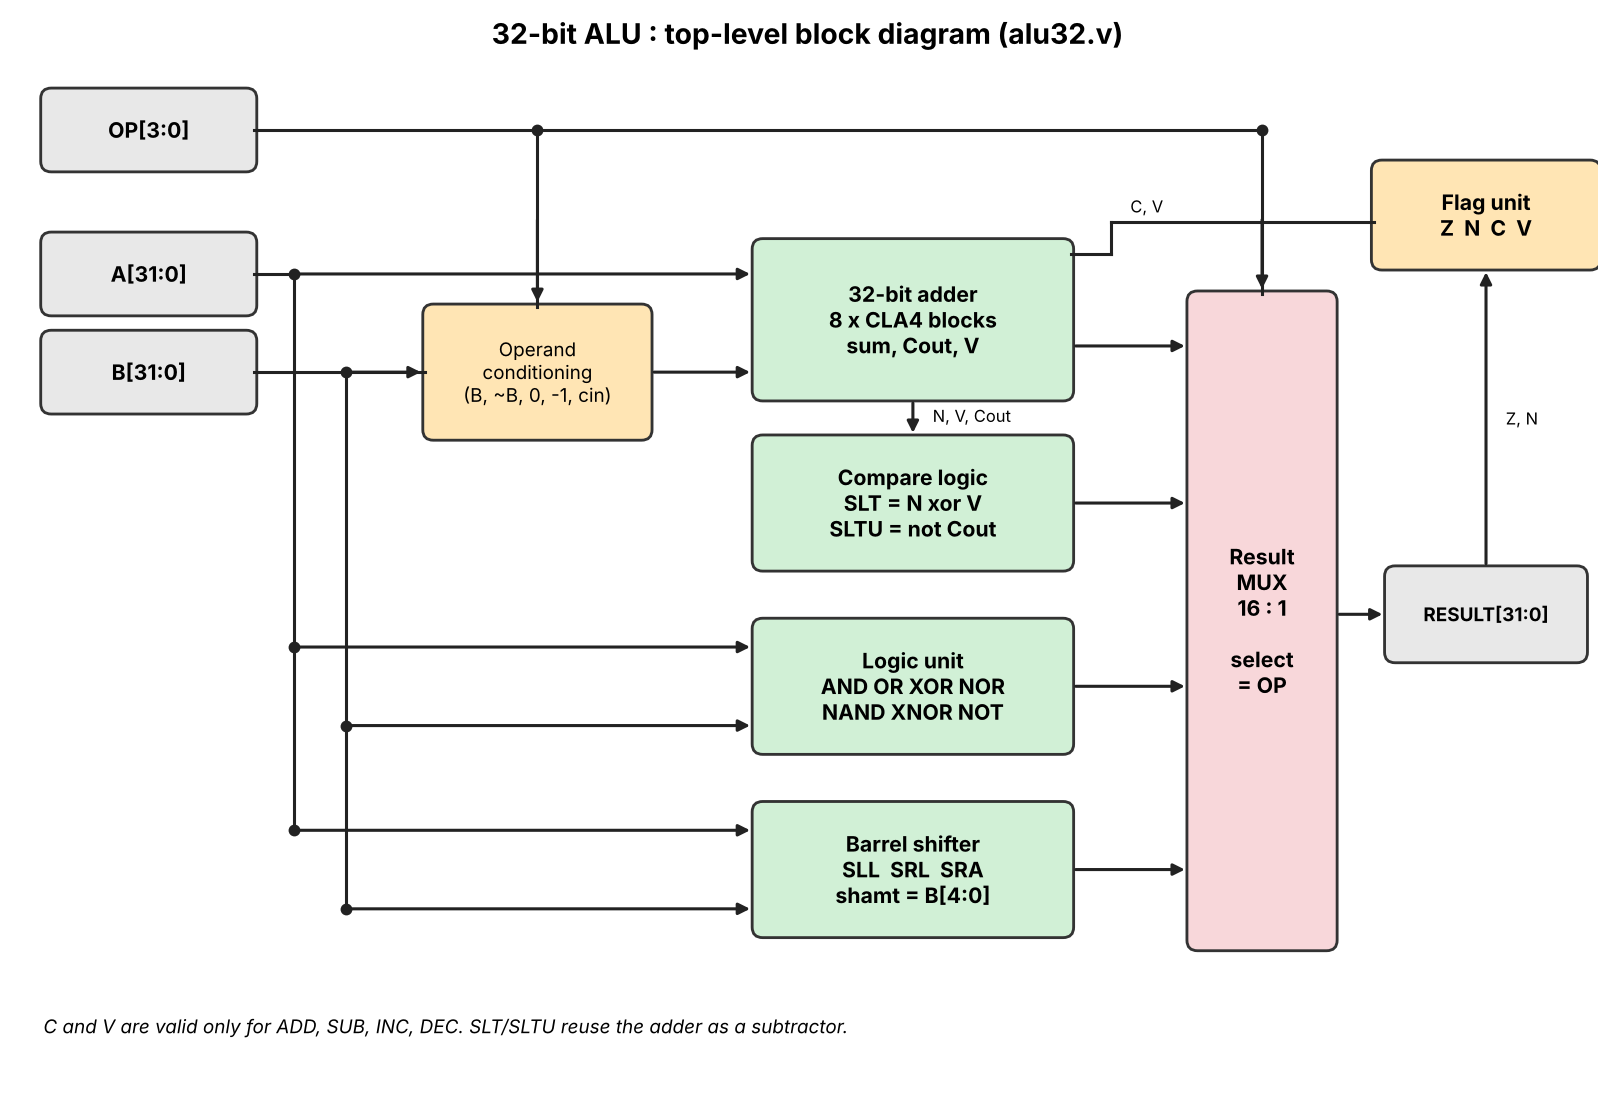
\includegraphics[width=\textwidth]{../docs/figures/alu_block_diagram.png}
\caption{Top-level block diagram of the 32-bit ALU.}\label{fig:top}
\end{figure}

\begin{table}[H]\centering
\begin{tabular}{@{}lcc@{}}\toprule
Operation & Adder $B$ input & Carry-in\\\midrule
ADD & $B$ & 0\\
SUB, SLT, SLTU & $\overline{B}$ & 1\\
INC & 0 & 1\\
DEC & \texttt{0xFFFFFFFF} & 0\\\bottomrule
\end{tabular}
\caption{Operand conditioning for the shared adder.}
\end{table}

\subsection{Adder}
\begin{figure}[H]\centering
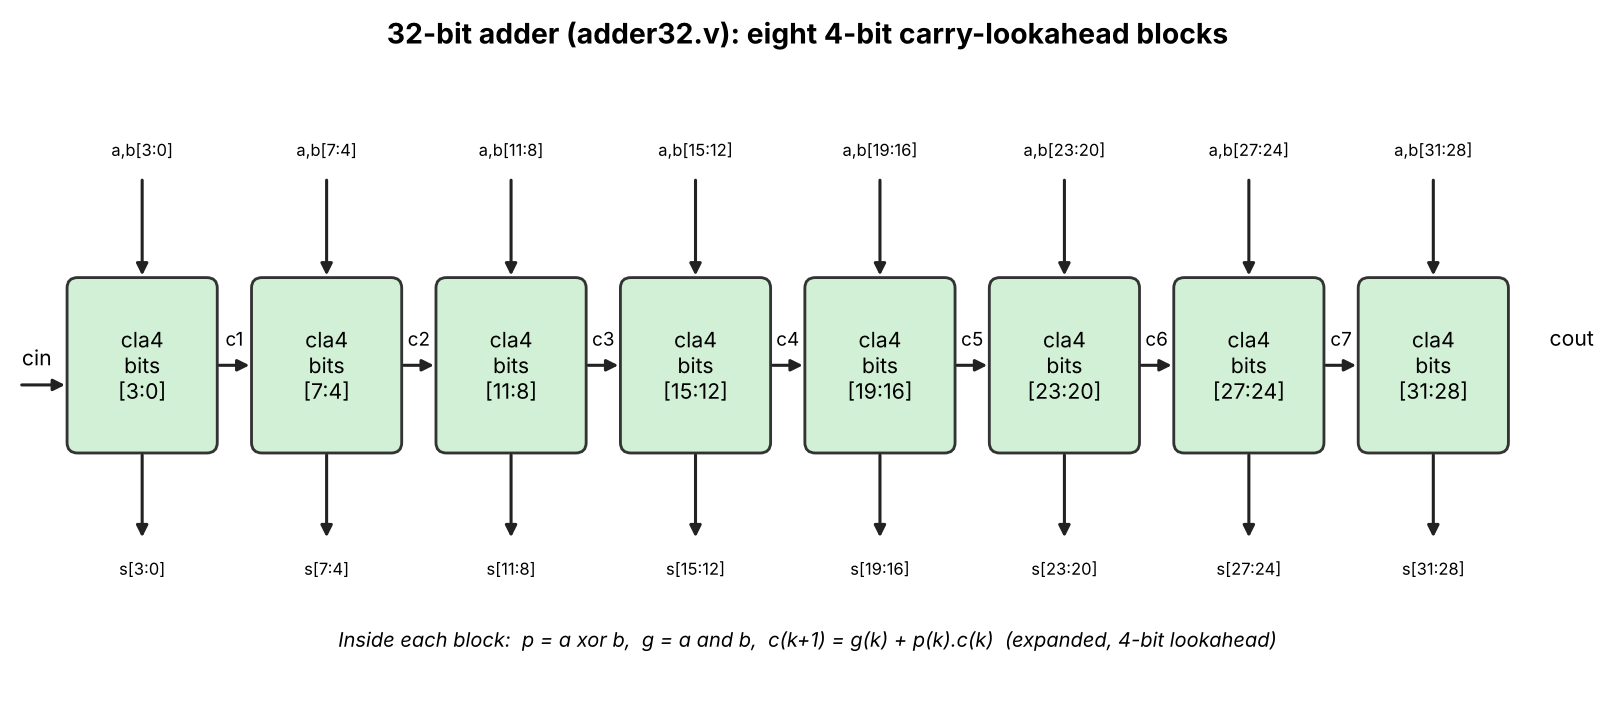
\includegraphics[width=\textwidth]{../docs/figures/adder_cla.png}
\caption{32-bit adder built from eight 4-bit carry-lookahead blocks.}
\end{figure}
Signed overflow is detected as $V = (a_{31}=b'_{31}) \wedge (s_{31}\neq a_{31})$, where $b'$ is the operand actually presented to the adder. This one expression is correct for ADD, SUB (where $b'=\overline{B}$), INC and DEC.

\subsection{Barrel shifter}
\begin{figure}[H]\centering
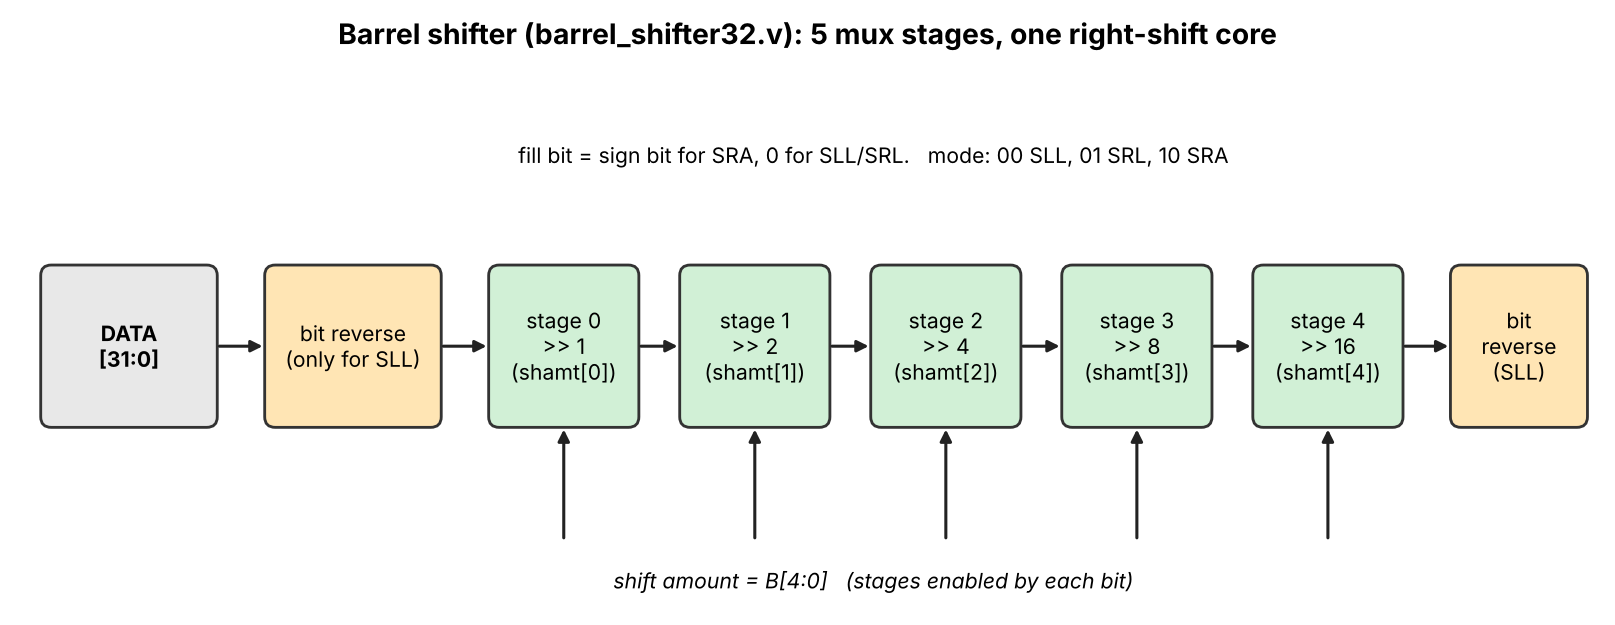
\includegraphics[width=\textwidth]{../docs/figures/barrel_shifter.png}
\caption{Five-stage barrel shifter with bit reversal for left shifts.}
\end{figure}

%------------------------------------------------------------
\section{Verilog implementation}
The design is split into four modules, listed in Table~\ref{tab:mods}. The complete source code is given in Appendix~A.
\begin{table}[H]\centering
\begin{tabular}{@{}lll@{}}\toprule
Module & File & Role\\\midrule
\texttt{alu32} & \texttt{rtl/alu32.v} & Top module: conditioning, result mux, compare, flags\\
\texttt{adder32} & \texttt{rtl/adder32.v} & Eight \texttt{cla4} blocks chained by carry\\
\texttt{cla4} & \texttt{rtl/adder32.v} & 4-bit carry-lookahead block\\
\texttt{barrel\_shifter32} & \texttt{rtl/barrel\_shifter32.v} & SLL, SRL and SRA\\\bottomrule
\end{tabular}
\caption{Module hierarchy.}\label{tab:mods}
\end{table}
Design decisions worth noting: the adder is structural (a \texttt{generate} loop of \texttt{cla4} instances) so that the lookahead logic is visible; the result multiplexer is a single \texttt{case} statement with a default that returns zero; and the code uses only Verilog-2005 constructs and no vendor primitives, so it is portable across simulators and synthesis tools.

%------------------------------------------------------------
\section{Verification}
\subsection{Method}
The system testbench \texttt{tb\_alu32} contains a behavioural reference model that is deliberately written differently from the RTL. It uses the simulator's own \texttt{+}, \texttt{-}, shift and comparison operators, and finds signed overflow by comparing bits 33 and 32 of a 34-bit sign-extended result. A second, independent check is provided by a Python model whose output is stored in \texttt{tb/vectors.mem} and read by the testbench. For every vector the result and all four flags are compared.

\subsection{Test plan}
\begin{table}[H]\centering\small
\begin{tabular}{@{}llp{8.2cm}@{}}\toprule
ID & Test & Purpose\\\midrule
T1 & Known answers & Sums, differences, carry, overflow, borrow, signed and unsigned compare, SRA\\
T2 & Corner $\times$ corner & All 16 operations on every pair of 8 corner values\\
T3 & All shift amounts & SLL, SRL, SRA for shift 0 to 31; upper bits of $B$ ignored\\
T4 & Constrained random & 20,000 operations, 25\% of operands biased to corner values\\
T5 & Golden vectors & 3,100 vectors from the Python model\\
U1 & \texttt{cla4} exhaustive & All 512 combinations of 4-bit inputs and carry-in\\
U2 & \texttt{adder32} random & Carry ripple across all 8 blocks, 20,000 random additions\\
U3 & \texttt{barrel\_shifter32} & Every shift amount and mode on several patterns plus random data\\\bottomrule
\end{tabular}
\caption{Test plan.}
\end{table}

\subsection{Golden-model cross-check}
The Python script \texttt{sw/ref\_model.py} contains two models: a plain-integer reference, and a bit-level emulation of the RTL structure (the \texttt{cla4} chain, the five-stage shifter, the $N\oplus V$ comparison and the flag masking). The two agree on all 3,100 golden vectors and on a further 200,000 random vectors, with zero mismatches. This confirms the logic equations used in the Verilog; it does not replace running the Verilog testbenches.

\subsection{Known-answer tests}
Table~\ref{tab:kat} lists a representative set of expected results produced by the golden model. These are the values the testbench checks the hardware against.
\begin{table}[H]\centering\small
\begin{tabular}{@{}lccccccc@{}}\toprule
Op & A & B & Result & N & Z & C & V\\\midrule
\texttt{ADD} & \texttt{0000000A} & \texttt{00000014} & \texttt{0000001E} & 0 & 0 & 0 & 0 \\
\texttt{ADD} & \texttt{FFFFFFFF} & \texttt{00000001} & \texttt{00000000} & 0 & 1 & 1 & 0 \\
\texttt{ADD} & \texttt{7FFFFFFF} & \texttt{00000001} & \texttt{80000000} & 1 & 0 & 0 & 1 \\
\texttt{SUB} & \texttt{00000032} & \texttt{00000014} & \texttt{0000001E} & 0 & 0 & 1 & 0 \\
\texttt{SUB} & \texttt{00000005} & \texttt{0000000A} & \texttt{FFFFFFFB} & 1 & 0 & 0 & 0 \\
\texttt{SUB} & \texttt{80000000} & \texttt{00000001} & \texttt{7FFFFFFF} & 0 & 0 & 1 & 1 \\
\texttt{AND} & \texttt{F0F0F0F0} & \texttt{0FF00FF0} & \texttt{00F000F0} & 0 & 0 & 0 & 0 \\
\texttt{XOR} & \texttt{AAAAAAAA} & \texttt{55555555} & \texttt{FFFFFFFF} & 1 & 0 & 0 & 0 \\
\texttt{SLL} & \texttt{00000001} & \texttt{00000004} & \texttt{00000010} & 0 & 0 & 0 & 0 \\
\texttt{SRL} & \texttt{80000000} & \texttt{00000004} & \texttt{08000000} & 0 & 0 & 0 & 0 \\
\texttt{SRA} & \texttt{80000000} & \texttt{00000004} & \texttt{F8000000} & 1 & 0 & 0 & 0 \\
\texttt{SLT} & \texttt{FFFFFFFF} & \texttt{00000001} & \texttt{00000001} & 0 & 0 & 0 & 0 \\
\texttt{SLTU} & \texttt{FFFFFFFF} & \texttt{00000001} & \texttt{00000000} & 0 & 1 & 0 & 0 \\
\texttt{INC} & \texttt{7FFFFFFF} & \texttt{00000000} & \texttt{80000000} & 1 & 0 & 0 & 1 \\
\texttt{DEC} & \texttt{00000000} & \texttt{00000000} & \texttt{FFFFFFFF} & 1 & 0 & 0 & 0 \\
\texttt{NOT} & \texttt{0000FFFF} & \texttt{00000000} & \texttt{FFFF0000} & 1 & 0 & 0 & 0 \\
\bottomrule
\end{tabular}
\caption{Expected results for selected operations (hexadecimal).}\label{tab:kat}
\end{table}

%------------------------------------------------------------
\section{Simulation and synthesis}
\subsection{Running the simulation}
From the project root, \texttt{sh run\_sim.sh} (Linux/macOS) or \texttt{run\_sim.bat} (Windows) compiles and runs the three testbenches with Icarus Verilog. Each testbench ends with the line \texttt{>>> ALL TESTS PASSED <<<} when every check succeeds, and \texttt{tb\_alu32} also prints a coverage line giving the number of checks per operation. The waveform is saved as \texttt{sim/alu32.vcd} and can be opened with GTKWave.

\subsection{Simulation results}
\begin{figure}[H]\centering
\fbox{\parbox{0.85\textwidth}{\centering\vspace{2.2cm}
\textbf{[Insert screenshot of the testbench console output here]}\vspace{2.2cm}}}
\caption{Console output of \texttt{run\_sim} showing all tests passed.}
\end{figure}
\begin{figure}[H]\centering
\fbox{\parbox{0.85\textwidth}{\centering\vspace{2.2cm}
\textbf{[Insert GTKWave screenshot of \texttt{sim/alu32.vcd} here]}\vspace{2.2cm}}}
\caption{Waveform of \texttt{a}, \texttt{b}, \texttt{op}, \texttt{result} and the flags.}
\end{figure}

\subsection{Synthesis}
The scripts \texttt{synth/synth\_generic.ys} and \texttt{synth/synth\_ecp5.ys} synthesise the design with Yosys to a generic 2-input gate library and to Lattice ECP5 LUTs respectively; \texttt{sh run\_synth.sh} runs both and writes the statistics to \texttt{synth/reports/}.

%------------------------------------------------------------
\section{Conclusion and future work}
A 32-bit ALU with sixteen operations and four status flags was designed in modular Verilog-2005. Sharing one adder between addition, subtraction, increment, decrement and both comparisons keeps the hardware small, and the carry-lookahead blocks and barrel shifter give predictable, parallel structures. The verification setup combines an independent reference model, directed and random tests, and golden vectors from a second model written in Python.

Possible extensions are a two-level lookahead adder to shorten the carry path, a hardware multiplier and divider, a registered (pipelined) version with a clock, and integration of the ALU into a simple processor datapath.

\begin{thebibliography}{9}
\bibitem{mano} M. M. Mano and M. D. Ciletti, \emph{Digital Design: With an Introduction to the Verilog HDL}, 5th ed., Pearson, 2013.
\bibitem{parhami} B. Parhami, \emph{Computer Arithmetic: Algorithms and Hardware Designs}, 2nd ed., Oxford University Press, 2010.
\bibitem{ph} D. A. Patterson and J. L. Hennessy, \emph{Computer Organization and Design RISC-V Edition}, 2nd ed., Morgan Kaufmann, 2020.
\bibitem{ieee} \emph{IEEE Standard for Verilog Hardware Description Language}, IEEE Std 1364-2005.
\bibitem{yosys} C. Wolf, \emph{Yosys Open SYnthesis Suite}, \url{https://yosyshq.net/yosys/}.
\end{thebibliography}

\appendix
\section{Verilog source code}
\subsection{alu32.v}
\lstinputlisting{../rtl/alu32.v}
\subsection{adder32.v}
\lstinputlisting{../rtl/adder32.v}
\subsection{barrel\_shifter32.v}
\lstinputlisting{../rtl/barrel_shifter32.v}
\subsection{tb\_alu32.v}
\lstinputlisting{../tb/tb_alu32.v}
\end{document}
